% Provenance (never printed): old seconde/premiere S material on water as a
% resource (stocks and flows of the water cycle, residence times, groundwater,
% overuse as a physical fact); see sources/book2/PROVENANCE.md. Residence
% times are computed in figdata/grade-10/residence_times.py, the Aral Sea
% budget in figdata/grade-10/aral_sea.py.
\chapter{موارد المياه العذبة}\label{ch:g10:freshwater-resources}

في عام 1960 كان بحر آرال، في صحارى آسيا الوسطى، رابع أكبر بحيرة في العالم. وكان
يصب فيه نهران عظيمان، تغذيهما الثلوج والأمطار في جبال بعيدة؛ ولا يخرج منه أي نهر.
وفي ستينيات القرن العشرين حُوّل ماؤهما لري الصحراء. وقد رصدت الأقمار الصناعية ما
تلا ذلك: انقسمت البحيرة أجزاءً، وصار معظم قاعها اليوم أرضًا جافة. ولم يكن السبب،
في الغالب الأعظم، تغيرًا في المناخ بل الري: فقد تلقت البحيرة من الماء أقل بكثير مما
كان التبخر يأخذه منها كل سنة. يحصي هذا الفصل مياه الأرض، وأين تُخزن وبأي سرعة
تتحرك، ويبيّن أن مورد الماء هو قبل كل شيء \omterm{def:g10:freshwater-resources:stock}{دفق}: فحين يؤخذ من خزان أكثر مما يرد
إليه، يفرغ الخزان، بمعدل تتنبأ به ميزانية بسيطة.
% ledger: nasa:aral, gaybullaev:aral-1960, micklin:aral

\begin{omfigure}
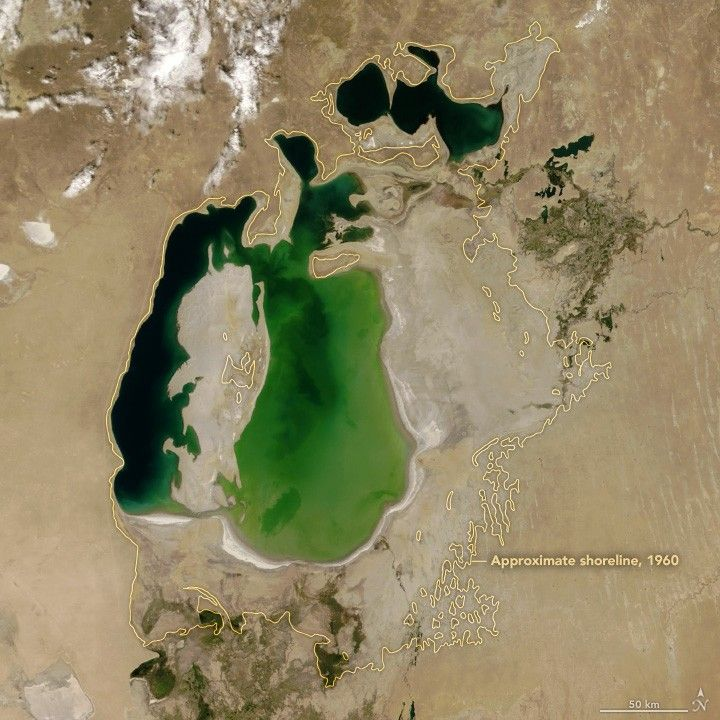
\includegraphics[width=0.47\linewidth]{images/book2/g10-nasa-aral-2000.jpg}\hspace{0.03\linewidth}%
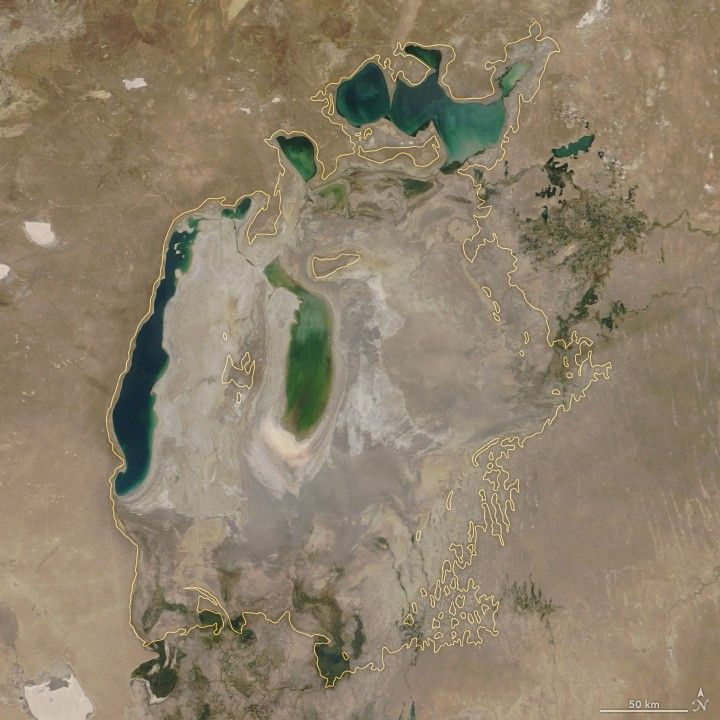
\includegraphics[width=0.47\linewidth]{images/book2/g10-nasa-aral-2018.jpg}

{\small بحر آرال كما رآه جهاز \babelsublr{MODIS} على متن القمر الصناعي تيرا التابع
لناسا في أغسطس 2000 (في اليمين) وأغسطس 2018 (في اليسار)؛ والخط الأصفر هو خط الشاطئ
التقريبي لعام 1960. ومسطرة المقياس \qty{50}{km}. الصور: مرصد الأرض التابع
لناسا.}
\end{omfigure}

\begin{recall}
تنقل الدورة المائية الماء بين المحيط والهواء واليابسة: تبخر، فتكاثف في سحب، فهطول،
فجريان سطحي؛ وكتلة الماء الكلية محفوظة (كتب الفيزياء). والصخور ذات المسام المتصلة
نفوذة؛ وتحت منسوب المياه الجوفية تمتلئ مسامها بالماء، والطبقة التي تحفظ من الماء
وتمرره ما يكفي لتغذية الآبار طبقة حاملة للمياه
(الكتاب 1، الصف 6). ومعظم مياه الأرض مياه مالحة (الكتاب 1،
الصف 2). ويحمل النهر ماء حوض تصريفه بعيدًا؛ وتصريفه
حجم في الثانية (\cref{ch:g10:drainage-basins}).
\end{recall}

\section{أين يوجد الماء}

تحوي الأرض نحو 1.39 مليار كيلومتر مكعب من الماء. ويوجد كله تقريبًا في المحيط؛
ولا يتجاوز العذب منه \qty{2.5}{\percent}. ومعظم هذا الماء العذب بعيد المنال: فأكثر
من ثلثيه متجمد في الغطاءات الجليدية والأنهار الجليدية، وقرابة ثلثه يقع تحت
الأرض.
% ledger: usgs:water-stocks

\begin{center}
\small
\begin{tabular}{|l|r|r|}
\hline
\textbf{الخزان} & \textbf{الحجم (\unit{km^3})} & \textbf{الحصة من الماء العذب} \\ \hline
المحيطات والبحار والخلجان & \num{1338000000} & (مالح) \\ \hline
الغطاءات الجليدية والأنهار الجليدية والثلوج الدائمة & \num{24064000} & \qty{68.7}{\percent} \\ \hline
المياه الجوفية العذبة & \num{10530000} & \qty{30.1}{\percent} \\ \hline
جليد التربة والتربة الصقيعية & \num{300000} & \qty{0.86}{\percent} \\ \hline
البحيرات العذبة & \num{91000} & \qty{0.26}{\percent} \\ \hline
رطوبة التربة & \num{16500} & \qty{0.05}{\percent} \\ \hline
الغلاف الجوي & \num{12900} & \qty{0.04}{\percent} \\ \hline
الأنهار & \num{2120} & \qty{0.006}{\percent} \\ \hline
\end{tabular}

{\small تقدير لمياه العالم، بحسب شيكلومانوف (1993)، عن هيئة المسح
الجيولوجي الأمريكية. وقد استُبعدت المياه الجوفية المالحة (\num{12870000}~\unit{km^3})
والبحيرات المالحة.}
\end{center}
% ledger: usgs:water-stocks

الأنهار والبحيرات العذبة، التي يستمد منها الناس معظم الماء الذي يستعملونه، لا تحوي
معًا إلا أقل من جزء من مئة من الواحد في المئة من كل الماء. ومع ذلك لا تجف الأنهار
طويلًا: فهي ليست \omterm{def:g10:freshwater-resources:stock}{مخزونًا} بل \omterm{def:g10:freshwater-resources:stock}{دفق}، يتجدد مع كل
مطر.

\section{المخزونات والدفوق}

\begin{definition}[المخزون؛ الدفق]\label{def:g10:freshwater-resources:stock}
في ميزانية مائية، \emph{المخزون}\index{مخزون (من الماء)} هو كمية الماء
المحفوظة في خزان --- المحيط، أو الهواء، أو الجليد، أو طبقة حاملة للمياه، أو بحيرة
--- في لحظة معينة، معبَّرًا عنها بحجم أو كتلة.
و\emph{الدفق}\index{دفق (من الماء)} هو الكمية التي تنتقل من خزان إلى آخر في وحدة
الزمن، بالكيلومترات المكعبة في السنة مثلًا.
\end{definition}

لا يتغير \omterm{def:g10:freshwater-resources:stock}{المخزون} إلا عبر \omterm{def:g10:freshwater-resources:stock}{دفوقه}: ما يدخل مطروحًا منه ما يخرج. وحين يتساويان، يكون
\omterm{def:g10:freshwater-resources:stock}{المخزون} في \emph{حالة ثبات}: إذ يبقى على حاله مع أن ماءه
يتجدد دائمًا.

\begin{omfigure}
\begin{tikzpicture}[font=\footnotesize, >={Stealth[length=6pt]}]
  % ocean, land, atmosphere
  \fill[omSea] (0,0) rectangle (6.4,1.6);
  \fill[omLithAlluv] (6.4,0) -- (6.4,1.6) -- (8.2,2.1) -- (10.4,2.6) -- (12,2.9) -- (12,0) -- cycle;
  \fill[omLithSand!60] (6.4,0) -- (12,0) -- (12,1.0) -- (6.4,0.7) -- cycle;
  \draw[black!50] (6.4,1.6) -- (8.2,2.1) -- (10.4,2.6) -- (12,2.9);
  \fill[omIce] (10.6,2.65) -- (11.3,3.35) -- (12,2.9) -- cycle;
  \node[align=center] at (3.2,0.75) {\textbf{المحيط}\\\num{1335040}};
  \node[align=center] at (9.3,1.35) {\foreignlanguage{arabic}{رطوبة التربة 122}\\\foreignlanguage{arabic}{البحيرات والأنهار 178}};
  \node[align=center] at (9.3,0.35) {\foreignlanguage{arabic}{المياه الجوفية \babelsublr{\num{15300}}}};
  \node[align=center] at (11.2,2.25) {الجليد\\\num{26350}};
  % atmosphere
  \draw[black!30, rounded corners=8pt, fill=omWxCloud] (1.0,4.6) rectangle (11.0,5.6);
  \node[align=center] at (6.0,5.1) {\foreignlanguage{arabic}{\textbf{الغلاف الجوي} 12.7}};
  % fluxes
  \draw[->, omProp, line width=1.4pt] (1.4,1.7) -- node[left, align=right] {تبخر\\413} (1.4,4.5);
  \draw[->, omWxRain, line width=1.4pt] (4.4,4.5) -- node[pos=0.3, right, align=left] {هطول\\373} (4.4,1.7);
  \draw[->, omWxRain, line width=1.4pt] (7.6,4.5) -- node[pos=0.7, left, align=right] {هطول\\113} (7.6,2.05);
  \draw[->, omProp, line width=1.4pt] (10.0,2.6) -- node[right, align=left] {التبخر\\\foreignlanguage{arabic}{والنتح 73}} (10.0,4.5);
  \draw[->, black!60, line width=1.2pt] (4.9,5.85) -- node[above] {\foreignlanguage{arabic}{بخار ماء منقول فوق اليابسة: 40}} (7.4,5.85);
  \draw[->, omRiver, line width=1.4pt] (7.6,1.2) -- node[above, inner sep=2pt] {\foreignlanguage{arabic}{الجريان 40}} (6.0,1.2);
\end{tikzpicture}

{\small الدورة المائية العالمية في تسعينيات القرن العشرين (رسم تخطيطي؛ بغير مقياس).
\omterm{def:g10:freshwater-resources:stock}{المخزونات} بآلاف \unit{km^3}، \omterm{def:g10:freshwater-resources:stock}{والدفوق} بآلاف \unit{km^3} في السنة.
بحسب ترينبرث وآخرين (2007). وتختلف تقديرات \omterm{def:g10:freshwater-resources:stock}{المخزونات} من دراسة إلى أخرى:
قارن المياه الجوفية والجليد هنا بالجدول السابق.}
\end{omfigure}
% ledger: trenberth:water-cycle

الدورة متوازنة. ففي كل سنة يفقد المحيط \num{413000}~\unit{km^3} بالتبخر ويستعيد
\num{373000} مطرًا وثلجًا و\num{40000} من الأنهار. ويتلقى الهواء
$413\,000 + 73\,000 = \num{486000}$~\unit{km^3}
ويعيد $373\,000 + 113\,000$، أي القدر نفسه. وتتلقى اليابسة
\num{113000}~\unit{km^3} من الهطول؛ يعود منها \num{73000} إلى الهواء بالتبخر
وعبر أوراق النباتات، ويجري الباقي، \num{40000}، إلى البحر، في الأنهار
وتحت الأرض.
% ledger: trenberth:water-cycle

\begin{definition}[المياه العذبة المتجددة]\label{def:g10:freshwater-resources:renewable}
\emph{المياه العذبة المتجددة}\index{مياه عذبة متجددة} لمنطقة هي \omterm{def:g10:freshwater-resources:stock}{دفق} الماء العذب
الذي يجدده الهطول كل سنة، والذي يمر عبرها جريانًا في الأنهار ومياهًا جوفية. إنها
\omterm{def:g10:freshwater-resources:stock}{دفق}، بالكيلومترات المكعبة في السنة، لا \omterm{def:g10:freshwater-resources:stock}{مخزون}.
\end{definition}

لليابسة كلها، هي \num{40000}~\unit{km^3} التي تبلغ البحر كل سنة. وتستطيع
منطقة أن تستعمل مياهها المتجددة سنة بعد سنة دون أن ينقصها الماء. وما تأخذه فوقها لا
يمكن أن يأتي إلا من \omterm{def:g10:freshwater-resources:stock}{مخزون}، يتقلص
عندئذ.

\section{زمن المكوث}

كم تبقى جزيئة ماء في خزان؟ بعضها يغادر فورًا، وبعضها يبقى زمنًا أطول بكثير؛ لكن
الإجابة في المتوسط تنتج من \omterm{def:g10:freshwater-resources:stock}{المخزون} \omterm{def:g10:freshwater-resources:stock}{والدفق}
وحدهما.

\begin{definition}[زمن المكوث]\label{def:g10:freshwater-resources:residence-time}
\emph{زمن المكوث}\index{زمن المكوث} للماء في خزان هو متوسط الزمن الذي يقضيه
الماء فيه بين دخوله وخروجه.
\end{definition}

\begin{proposition}[زمن المكوث والمخزون والدفق]\label{prop:g10:freshwater-resources:residence}
لخزان في حالة ثبات، يحوي \omterm{def:g10:freshwater-resources:stock}{مخزونًا} $S$ ويعبره \omterm{def:g10:freshwater-resources:stock}{دفق} $F$
(داخلًا وخارجًا)، \omterm{def:g10:freshwater-resources:residence-time}{زمن المكوث} هو
\[
T = \frac{S}{F}.
\]
\end{proposition}

\begin{proof}
في حالة الثبات، يدخل حجم $F$ ويخرج حجم $F$ كل سنة، بينما يبقى
\omterm{def:g10:freshwater-resources:stock}{المخزون} $S$. وبعد زمن $S/F$، يكون حجم $F \times S/F = S$ قد
دخل: أي قدر ما يحويه الخزان كله. وفي المتوسط يكون الماء الموجود في
البداية قد استُبدل حينئذ، فيبقى الماء $S/F$ في الخزان.
\end{proof}

\begin{example}[الماء في الهواء]\label{ex:g10:freshwater-resources:atmosphere}
يحوي الغلاف الجوي \num{12700}~\unit{km^3} من الماء، ويسقط منه
\num{486000}~\unit{km^3} كل سنة مطرًا وثلجًا. \omterm{def:g10:freshwater-resources:residence-time}{وزمن
مكوثه} $12\,700/486\,000 \approx \num{0.026}$ سنة، أي نحو
\num{9.5} أيام: فماء الهواء يتجدد كل أسبوع أو أسبوعين. والسحابة
التي تمطر اليوم مكوّنة من ماء غادر المحيط أو الأرض قبل بضعة
أيام.
\end{example}
% ledger: trenberth:water-cycle (t_atmosphere_days 9.5 in figdata/grade-10/residence_times.py)

ويعطي الحساب نفسه نحو \num{19} يومًا للماء في مجاري الأنهار
($2120$~\unit{km^3} يحملها \num{40000}~\unit{km^3} في السنة)، وبضع
سنوات للبحيرات والأنهار معًا، ونحو \num{3200} سنة للمحيط
($1\,335\,040/413$ ألف~\unit{km^3}). وقد تكون المياه الجوفية أبطأ أيضًا: فأعمق
مياه بعض الطبقات الحاملة للمياه عمرها مئات آلاف السنين.
% ledger: trenberth:water-cycle, usgs:water-stocks, sturchio:nubian-age

\begin{omfigure}
\begin{tikzpicture}
\begin{axis}[omrecord, xbar, xmode=log, log origin=infty, width=0.74\linewidth, height=5.6cm,
  xmin=1, xmax=1e9, ymin=-0.6, ymax=4.6, bar width=11pt,
  ytick={0,1,2,3,4}, yticklabels={الغلاف الجوي, الأنهار, {البحيرات والأنهار}, المحيط, {عمر المياه الجوفية العميقة}},
  xtick={1,30.44,365.25,36525,3652500,365250000}, xticklabels={{يوم واحد}, {شهر واحد}, {سنة واحدة}, {\foreignlanguage{arabic}{\mbox{\textdir TLT 100} سنة}}, {\foreignlanguage{arabic}{\num{10000} سنة}}, {مليون سنة}},
  xticklabel style={font=\scriptsize, rotate=25, anchor=north east}, yticklabel style={font=\small},
  xlabel={\foreignlanguage{arabic}{زمن المكوث، بمقياس لوغاريتمي}}, label style={font=\small}, xmajorgrids]
\addplot[fill=omDef!45, draw=omDef!80!black] table[x=days, y=idx] {figdata/out/grade-10-residence_times-times.dat};
\draw[fill=omProp!45, draw=omProp!80!black] (axis cs:73050000,3.75) rectangle (axis cs:365250000,4.25);
\node[anchor=west, font=\scriptsize] at (axis cs:9.5,0) {\foreignlanguage{arabic}{\babelsublr{\num{9.5}} أيام}};
\node[anchor=west, font=\scriptsize] at (axis cs:19.4,1) {\foreignlanguage{arabic}{\babelsublr{\num{19}} يومًا}};
\node[anchor=west, font=\scriptsize] at (axis cs:1625,2) {\foreignlanguage{arabic}{\babelsublr{\num{4.5}} سنوات}};
\node[anchor=west, font=\scriptsize] at (axis cs:1180690,3) {\foreignlanguage{arabic}{\babelsublr{\num{3200}} سنة}};
\node[anchor=east, font=\scriptsize] at (axis cs:73050000,4) {\foreignlanguage{arabic}{من \babelsublr{\num{200000}} إلى مليون سنة}};
\end{axis}
\end{tikzpicture}

{\small \omterm{def:g10:freshwater-resources:residence-time}{أزمنة مكوث} الماء، محسوبة بقسمة \omterm{def:g10:freshwater-resources:stock}{المخزون} على \omterm{def:g10:freshwater-resources:stock}{الدفق} في الدورة المائية
العالمية (بالأزرق)، والعمر المقيس للمياه الجوفية العميقة تحت شرق الصحراء الكبرى
(بالبرتقالي). محور لوغاريتمي: بدءًا من السنة الواحدة، كل خطوة معلَّمة مئة ضعف. البيانات:
ترينبرث وآخرون (2007)؛ هيئة المسح الجيولوجي الأمريكية؛ ستورتشيو وآخرون
(2004).}
\end{omfigure}
% values computed in figdata/grade-10/residence_times.py

يقيس \omterm{def:g10:freshwater-resources:residence-time}{زمن المكوث} سرعة تعافي الخزان. فالماء المأخوذ من نهر يُعوَّض في أيام؛ والبحيرة
الملوثة أو المفرغة تحتاج إلى سنوات؛ والمياه الجوفية التي استغرق تجمعها آلاف السنين
لا تتجدد إطلاقًا على مقياس حياة
الإنسان.

\begin{method}[ميزانية مائية]\label{met:g10:freshwater-resources:budget}
\begin{enumerate}
  \item اختر الخزان: بحيرة، أو طبقة حاملة للمياه، أو حوضًا، أو الهواء.
  \item اسرد كل \omterm{def:g10:freshwater-resources:stock}{دفق} داخل إليه (الأنهار، المطر، التسرب) وخارج منه
        (الأنهار، التبخر، الضخ)، بالوحدة نفسها.
  \item تغيّر \omterm{def:g10:freshwater-resources:stock}{المخزون} في السنة هو مجموع المداخل مطروحًا منه
        مجموع المخارج.
  \item إذا لم يتغير \omterm{def:g10:freshwater-resources:stock}{المخزون}، تساوت المداخل والمخارج، وكان \omterm{def:g10:freshwater-resources:residence-time}{زمن
        المكوث} هو \omterm{def:g10:freshwater-resources:stock}{المخزون} مقسومًا على أي منهما.
\end{enumerate}
\end{method}

\section{الطبقات الحاملة للمياه خزاناتٍ}

المطر الذي يتسرب في الأرض ويبلغ منسوب المياه الجوفية \emph{يغذي}
الطبقة الحاملة للمياه التي تحته. ثم يتحرك الماء ببطء عبر مسام الصخر،
نحو الينابيع أو الأنهار أو البحر. وحيث تنغمس
طبقة نفوذة تحت طبقة كتيمة، كالطين، يكون ماؤها
\emph{محصورًا}: فلا يُغذّى إلا حيث تبلغ الطبقة السطح، وقد يكون ذلك
بعيدًا.

\begin{omfigure}
\begin{tikzpicture}[font=\footnotesize, >={Stealth[length=5pt]}]
  % layers dipping to the right
  \fill[lith shale] (0,0) -- (12,0) -- (12,0.8) -- (0,2.4) -- cycle;
  \fill[lith sandstone] (0,2.4) -- (12,0.8) -- (12,2.2) -- (2.2,3.5) -- (0,3.8) -- cycle;
  \fill[lith shale] (2.2,3.5) -- (12,2.2) -- (12,3.4) -- (3.6,3.9) -- cycle;
  % ground surface
  \draw[line width=0.8pt, brown!60!black] (0,3.8) -- (1.2,4.0) -- (2.2,3.9) -- (3.6,3.9) -- (6,3.6) -- (9,3.5) -- (12,3.4);
  \fill[omLithAlluv] (0,3.8) -- (1.2,4.0) -- (2.2,3.9) -- (2.2,3.5) -- (0,3.8) -- cycle;
  \fill[omLithAlluv] (2.2,3.9) -- (3.6,3.9) -- (2.2,3.5) -- cycle;
  \fill[omLithAlluv] (3.6,3.9) -- (6,3.6) -- (9,3.5) -- (12,3.4) -- (3.6,3.9) -- cycle;
  % water table in the unconfined part
  \draw[omDef, line width=1pt, dashed] (0,3.3) .. controls (1.0,3.35) and (1.8,3.2) .. (2.6,3.45);
  \node[anchor=south west, text=omDef, fill=white, fill opacity=0.8, text opacity=1, inner sep=1pt] at (0.05,2.75) {منسوب المياه الجوفية};
  % rain and recharge
  \foreach \x in {0.35,0.65,0.95,1.25} \draw[omWxRain, thick] (\x,4.9) -- (\x-0.15,4.4);
  \node[anchor=south, text=omWxRain] at (0.7,4.95) {المطر: تغذية};
  % flow arrows in the aquifer
  \draw[->, omDef, line width=1.1pt] (2.0,2.85) -- (4.4,2.55);
  \draw[->, omDef, line width=1.1pt] (5.4,2.4) -- (7.8,2.1);
  \draw[->, omDef, line width=1.1pt] (8.8,1.95) -- (11.2,1.65);
  % wells
  \draw[black!70, line width=1.6pt] (1.95,3.95) -- (1.95,2.9);
  \node[anchor=south] at (1.95,4.0) {بئر};
  \draw[black!70, line width=1.6pt] (7.0,3.55) -- (7.0,1.9);
  \node[anchor=south] at (7.0,3.6) {بئر};
  % labels
  \node[align=center, fill=white, fill opacity=0.85, text opacity=1, inner sep=1.5pt] at (1.5,0.8) {طين كتيم};
  \node[align=center, fill=white, fill opacity=0.85, text opacity=1, inner sep=1.5pt] at (8.6,2.95) {طين كتيم};
  \node[anchor=north, align=center] at (1.6,-0.1) {\foreignlanguage{arabic}{طبقة حاملة للمياه حرة:}\\منطقة التغذية};
  \node[anchor=north, align=center] at (6.4,-0.1) {طبقة حاملة للمياه محصورة};
  \node[anchor=north, align=center] at (10.6,-0.1) {ماء قديم، بعيد عن\\منطقة التغذية};
\end{tikzpicture}

{\small طبقة حاملة للمياه في حجر رملي نفوذ (رسم تخطيطي). يغذيها المطر
حيث تبلغ السطح؛ وهناك يكون منسوب المياه الجوفية حرًا في الارتفاع والانخفاض.
وأبعد من ذلك، تحت الطين، تكون الطبقة محصورة، ويتحرك ماؤها
ببطء نزولًا على امتدادها: وكلما ابتعد عن منطقة التغذية، كان الماء
أقدم.}
\end{omfigure}

\begin{definition}[المياه الجوفية الأحفورية]\label{def:g10:freshwater-resources:fossil-groundwater}
\emph{المياه الجوفية الأحفورية}\index{مياه جوفية أحفورية} مياه جوفية
دخلت طبقتها الحاملة منذ زمن بعيد، في الغالب تحت مناخ أرطب، ولا تجددها التغذية
الحالية على مقياس أعمار البشر.
\end{definition}

تحت شرق الصحراء الكبرى تمتد طبقة حاملة للمياه هائلة من الحجر الرملي. وأعمق مياهها،
المؤرَّخة بتحلل صورة مشعة نادرة من الكريبتون، يتراوح عمرها بين
\num{200000} سنة ومليون سنة. وقد تدفقت ببطء من منطقة تغذية
في جنوب غرب مصر، وتُظهر كيمياؤها أنها سقطت مطرًا في أثناء
فترات رطبة ماضية من العصور الجليدية، حين كان الهواء الرطب القادم من الأطلسي يبلغ
المنطقة. وهذا الماء، حين يُضخ اليوم، \omterm{def:g10:freshwater-resources:stock}{مخزون} يُستنزف، لا \omterm{def:g10:freshwater-resources:stock}{دفق}.
% ledger: sturchio:nubian-age

حين يتجاوز الضخ التغذية، ينخفض منسوب المياه الجوفية. ففي السهول العليا في
وسط الولايات المتحدة، تُضخ الطبقة الحاملة للمياه الممتدة تحت نحو \num{175000} ميل مربع
(\qty{453000}{km^2}) للري منذ نحو 1950. وبحلول 2015
كان منسوب مائها قد انخفض \qty{4.8}{m} في المتوسط، وحتى
\qty{71}{m} (234 قدمًا) في بعض الآبار؛ وكانت الطبقة قد فقدت نحو
\num{273} مليون أكر-قدم من الماء، أي نحو \qty{340}{km^3}.
% ledger: mcguire:high-plains (1 acre-foot = 1233.5 m3)

\begin{omfigure}
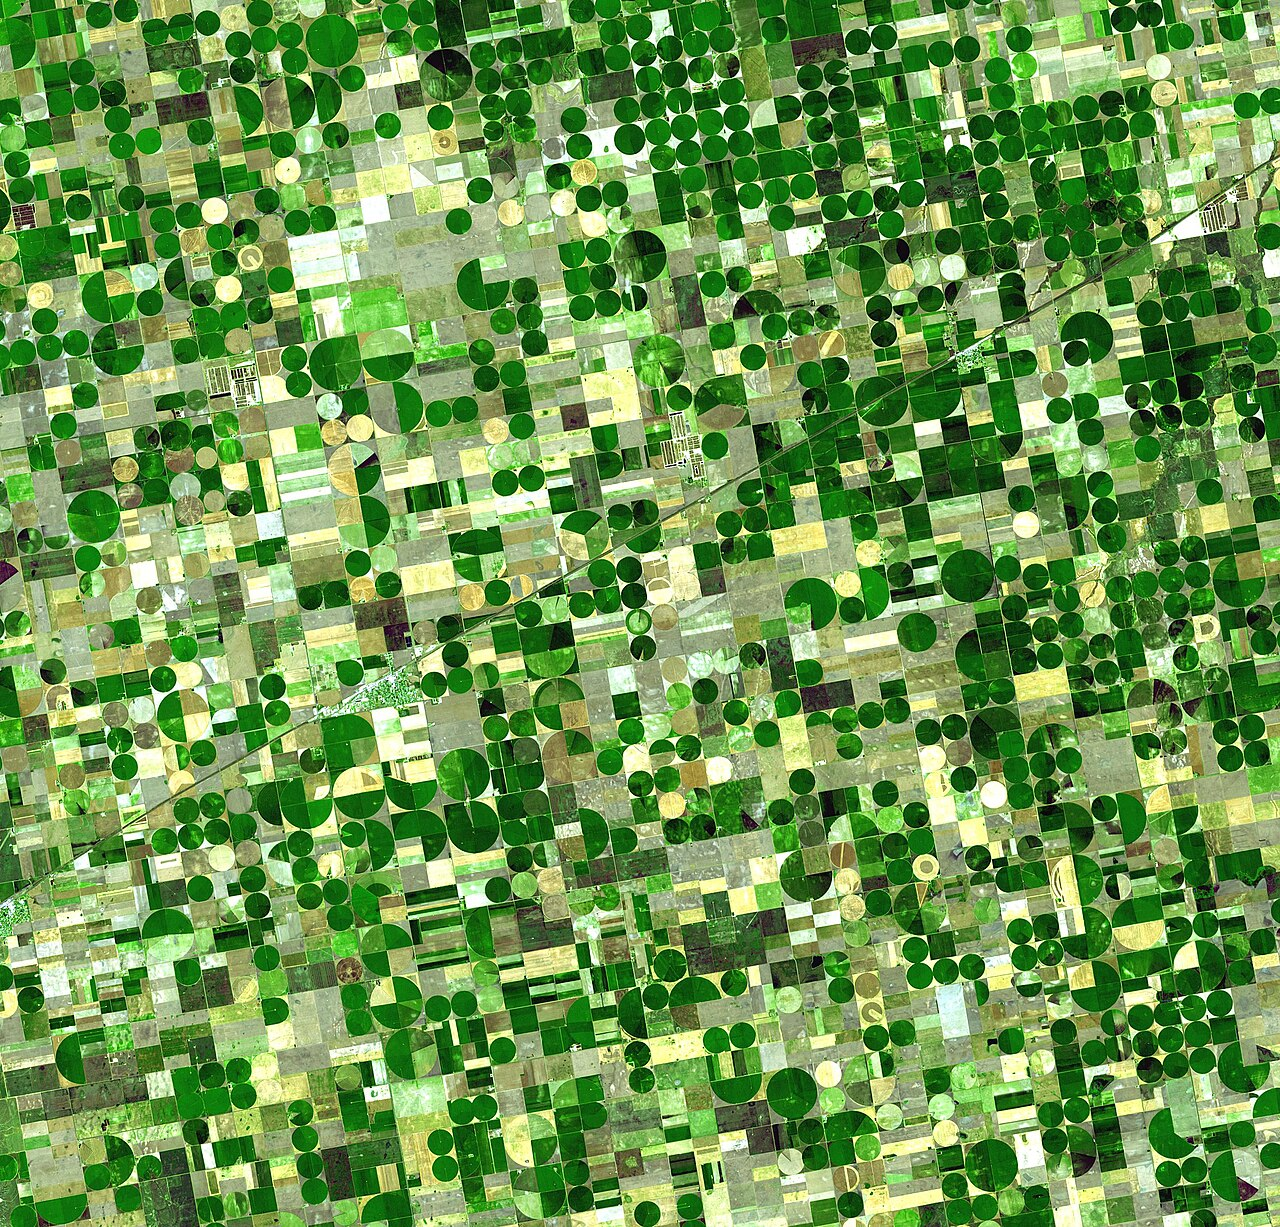
\includegraphics[width=0.5\linewidth]{images/book2/g10-nasa-kansas-center-pivot.jpg}

{\small حقول مروية قرب سابليت، كانساس، كما رآها جهاز \babelsublr{ASTER} على متن
القمر الصناعي تيرا التابع لناسا في يونيو 2001 (عرض المنظر نحو \qty{37}{km}). وكل دائرة
حقل يرويه ذراع رشاش طويل يدور حول مركزه؛ وأقطار
الدوائر \num{800} و\qty{1600}{m}. الصورة: ناسا (ملك عام).}
\end{omfigure}

لا يمكن رؤية المياه الجوفية من الفضاء، لكن يمكن وزنها: فقمران صناعيان
يطير أحدهما خلف الآخر يحسّان بالتغيرات الطفيفة في جذب الأرض التي تسببها
كتلة الماء التي تأتي وتذهب تحتهما، ويرسمان خريطة لأماكن ارتفاع \omterm{def:g10:freshwater-resources:stock}{مخزون} الماء
على اليابسة وانخفاضه من شهر إلى شهر.

\begin{omfigure}
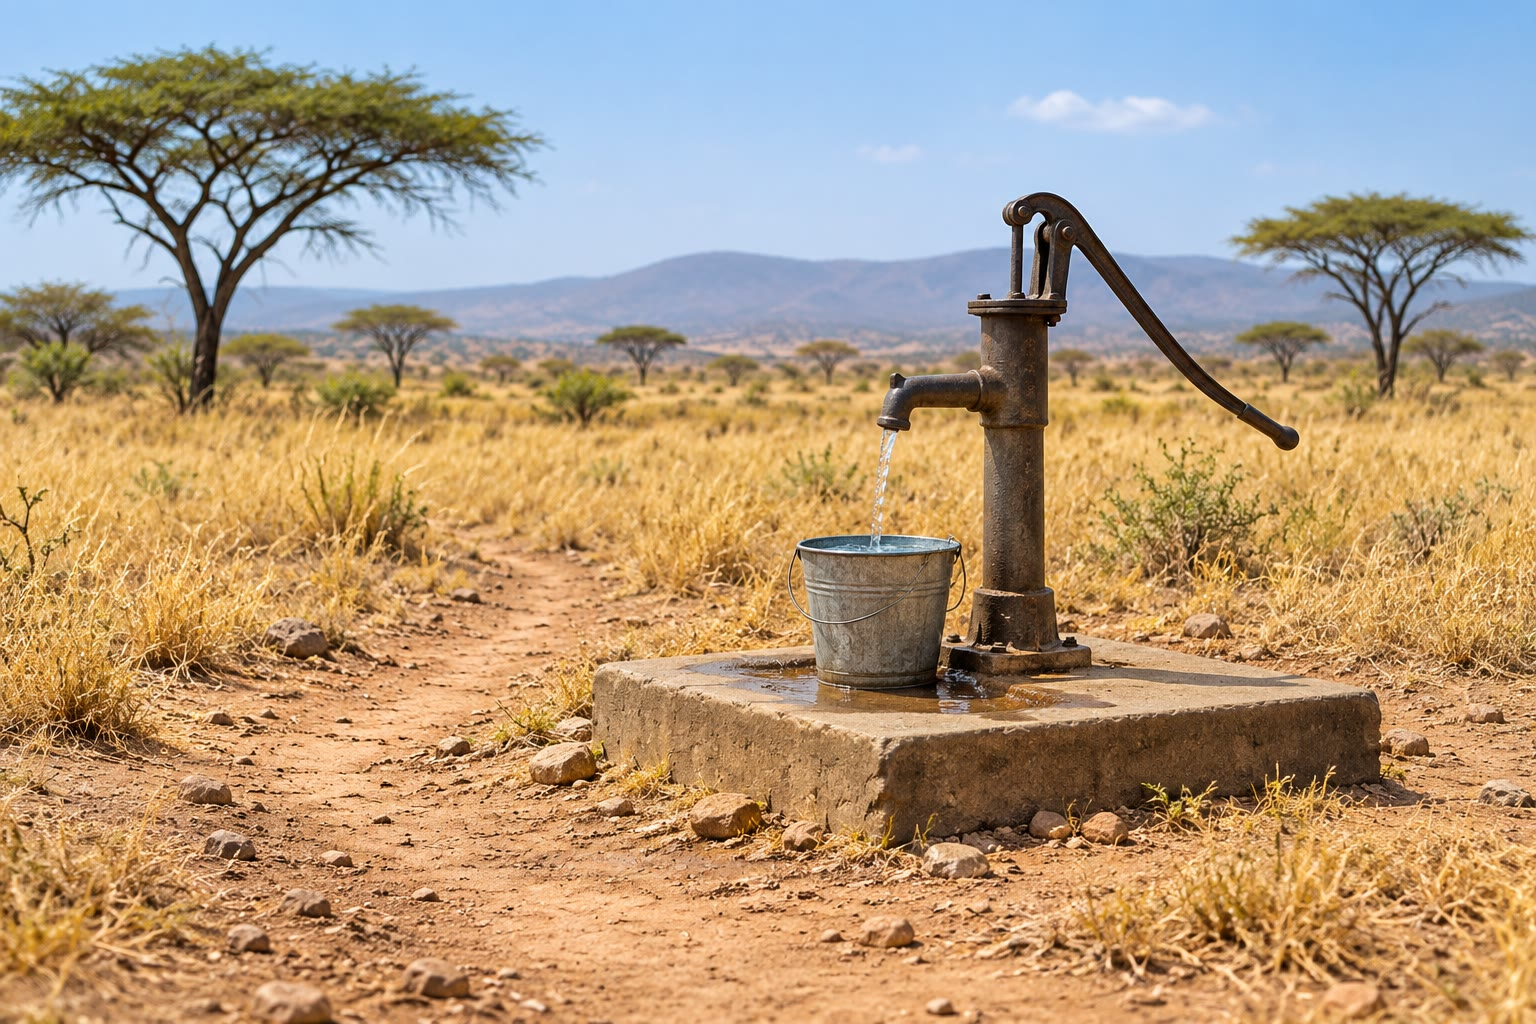
\includegraphics[width=0.55\linewidth]{images/book2/ai/g10-hand-pump-well.jpg}

{\small مضخة يدوية على بئر في منظر جاف: الماء المسحوب هنا يأتي
من الأرض تحتها، بعيدًا عن متناول موسم الجفاف.}
\end{omfigure}

\section{الإفراط في الاستعمال حقيقةً فيزيائية}

ليس لبحر آرال مخرج: فماء نهريه، آمو داريا
وسير داريا، لا يغادره إلا بالتبخر. وفي 1960 كان يغطي
\qty{68000}{km^2}، ويحوي \qty{1093}{km^3}، وكان ماؤه يحتوي على \qty{10}{g}
من الملح في اللتر. وفي تلك السنة أزال التبخر \qty{71.1}{km^3}، وجلب المطر الساقط
على البحيرة \qty{9.4}{km^3}: فلكي تحافظ البحيرة على منسوبها، كانت تحتاج إلى
$71.1 - 9.4 = \qty{61.7}{km^3}$ في السنة من نهريها.
% ledger: gaybullaev:aral-1960, gaybullaev:aral-table

منذ ستينيات القرن العشرين حُوّل النهران لري الصحراء، فلم يبلغ البحيرة من مائهما شيء
يُذكر تقريبًا: ففي السبعينيات والثمانينيات، كثيرًا ما كان أقل
من \qty{2}{km^3} في السنة. واستمر التبخر، فبدأت البحيرة
تتقلص. وميزانيتها تحدد سرعة ذلك. فالتبخر يأخذ طبقة من الماء
تتوقف سماكتها على المناخ، وهي هنا نحو متر في السنة
($71.1/68\,000 \approx \qty{0.00105}{km}$). فإذا توقف الوارد، انخفض المنسوب
بهذا القدر تقريبًا كل سنة، مطروحًا منه المطر. ومع تقلص البحيرة، تتقلص مساحتها
ومعها تبخرها، فيتباطأ الانخفاض؛ لكنه لا
يتوقف حتى يتوازن الوارد والتبخر من جديد.
% ledger: gaybullaev:aral-table (values computed in figdata/grade-10/aral_sea.py)

\begin{omfigure}
\begin{tikzpicture}
\begin{axis}[omrecord, name=vol, width=0.46\linewidth, height=5.4cm, xmin=1955, xmax=2012, ymin=0, ymax=1200,
  xtick={1960,1980,2000}, xticklabel style={/pgf/number format/1000 sep={}}, scaled y ticks=false,
  ylabel={\foreignlanguage{arabic}{الحجم \babelsublr{(\unit{km^3})}}}, xlabel={السنة}, tick label style={font=\small}, label style={font=\small},
  title={\small حجم الماء}]
\addplot[omDef, line width=1pt, mark=*, mark size=1.3pt] table[x=year, y=volume] {figdata/out/grade-10-aral_sea-record.dat};
\end{axis}
\begin{axis}[omrecord, at={(vol.east)}, anchor=west, xshift=1.4cm, width=0.46\linewidth, height=5.4cm,
  xmin=1955, xmax=2012, ymin=0, ymax=140, xtick={1960,1980,2000},
  xticklabel style={/pgf/number format/1000 sep={}},
  ylabel={\foreignlanguage{arabic}{الملوحة \babelsublr{(\unit{g/L})}}}, xlabel={السنة}, tick label style={font=\small}, label style={font=\small},
  title={\small الملوحة}]
\addplot[omProp, line width=1pt, mark=*, mark size=1.3pt] table[x=year, y=salinity] {figdata/out/grade-10-aral_sea-record.dat};
\end{axis}
\end{tikzpicture}

{\small بحر آرال من 1960 إلى 2010: انخفض حجم مائه إلى
العُشر، بينما صار الملح الذي خلّفه التبخر أشد تركيزًا بثلاث عشرة مرة. البيانات:
غايبولاييف وآخرون (2012).}
\end{omfigure}
% ledger: gaybullaev:aral-table

بحلول 2010 لم تعد البحيرة تحوي إلا \qty{98}{km^3}، أي عُشر حجمها في 1960، على مساحة
\qty{14280}{km^2}؛ وبلغت ملوحتها \qty{130}{g/L}، أي أشد ملوحة بكثير من
المحيط. وانخفض منسوبها بأكثر من \qty{20}{m}. ويهب غبار مالح
من القاع الجاف. والسبب غير خفي: فقد قُطع الوارد إلى البحيرة
بينما لم ينقطع تبخرها.
% ledger: gaybullaev:aral-table, gaybullaev:aral-1960, micklin:aral, nasa:aral

\section{تمارين}

\begin{exercise}[$\star$]\label{exo:g10:freshwater-resources:1}
عرّف \omterm{def:g10:freshwater-resources:stock}{المخزون} \omterm{def:g10:freshwater-resources:stock}{والدفق} \omterm{def:g10:freshwater-resources:residence-time}{وزمن المكوث}، وأعطِ وحدات كل منها.
\end{exercise}

\begin{exercise}[$\star$]\label{exo:g10:freshwater-resources:2}
من جدول مياه العالم: ما حصة الماء العذب من كل الماء؟ ومن الماء
العذب، ما حصتا المتجمد منه والجوفي؟ وأي خزان يحوي
أقله؟
\end{exercise}

\begin{exercise}[$\star$]\label{exo:g10:freshwater-resources:3}
عرّف \omterm{def:g10:freshwater-resources:renewable}{المياه العذبة المتجددة} \omterm{def:g10:freshwater-resources:fossil-groundwater}{والمياه الجوفية الأحفورية}. ولماذا تكون الأولى \omterm{def:g10:freshwater-resources:stock}{دفقًا}
والثانية \omterm{def:g10:freshwater-resources:stock}{مخزونًا}؟
\end{exercise}

\begin{exercise}[$\star$]\label{exo:g10:freshwater-resources:4}
كم مرة يزيد ما تحويه البحيرات العذبة في العالم (\num{91000}~\unit{km^3})
من الماء على ما تحويه أنهاره (\num{2120}~\unit{km^3})؟
\end{exercise}

\begin{exercise}[$\star$]\label{exo:g10:freshwater-resources:5}
على مخطط \omterm{def:g10:freshwater-resources:residence-time}{أزمنة المكوث}، أي خزان يجدد ماءه أسرع، وأيها
أبطأ؟ وكم مرة يطول بقاء الماء في المحيط عن بقائه في
الهواء؟
\end{exercise}

\begin{exercise}[$\star\star$]\label{exo:g10:freshwater-resources:6}
يحوي الغلاف الجوي \num{12700}~\unit{km^3} من الماء. احسب \omterm{def:g10:freshwater-resources:residence-time}{زمن مكوثه}
من التبخر الذي يدخله (\num{413000} من المحيط
و\num{73000}~\unit{km^3} من اليابسة كل سنة)، وتحقق من أنه يطابق
\omterm{def:g10:freshwater-resources:residence-time}{زمن المكوث} المحسوب من الهطول الذي يغادره.
\end{exercise}

\begin{exercise}[$\star\star$]\label{exo:g10:freshwater-resources:7}
يحوي المحيط \num{1335040} ألف~\unit{km^3} ويفقد
\num{413} ألف~\unit{km^3} في السنة بالتبخر. احسب \omterm{def:g10:freshwater-resources:residence-time}{زمن
مكوثه}. ولماذا يبقى هو نفسه إذا حُسب بما يدخله؟
\end{exercise}

\begin{exercise}[$\star\star$]\label{exo:g10:freshwater-resources:8}
باستعمال \omterm{def:g10:freshwater-resources:stock}{دفوق} الدورة المائية العالمية، اكتب ميزانية اليابسة: ما
يسقط عليها، وما يعود إلى الهواء، وما يجري. وما حصة المطر
الساقط على اليابسة التي تعود إلى الهواء؟
\end{exercise}

\begin{exercise}[$\star\star$]\label{exo:g10:freshwater-resources:9}
فقدت الطبقة الحاملة للمياه في السهول العليا نحو \num{273.2} مليون أكر-قدم من الماء
من نحو 1950 إلى 2015 (\num{1}~أكر-قدم = \qty{1233.5}{m^3}). حوّل
هذا الحجم إلى \unit{km^3} وقارنه بحجم بحر آرال في
1987 (\qty{345.6}{km^3}).
\end{exercise}

\begin{exercise}[$\star\star$]\label{exo:g10:freshwater-resources:10}
انخفض متوسط منسوب الماء في الطبقة الحاملة للمياه في السهول العليا \num{15.8} قدمًا
من نحو 1950 إلى 2015 (\num{1}~قدم = \qty{0.3048}{m}). فكم يساوي ذلك
بالأمتار، وبالسنتيمترات في السنة؟
\end{exercise}

\begin{exercise}[$\star\star$]\label{exo:g10:freshwater-resources:11}
طبقة حاملة للمياه تحوي \qty{2}{km^3} من الماء وتُغذّى بمقدار
\qty{0.01}{km^3} في السنة. ما \omterm{def:g10:freshwater-resources:residence-time}{زمن مكوث} مائها؟ والآبار الآن
تضخ منها \qty{0.05}{km^3} في السنة. افترض أن التغذية مستمرة وأن
الآبار صارت المخرج الوحيد للماء: فكم ستدوم
الطبقة؟
\end{exercise}

\begin{exercise}[$\star\star\star$]\label{exo:g10:freshwater-resources:12}
احسب \omterm{def:g10:freshwater-resources:residence-time}{زمن مكوث} ماء بحر آرال في 1960
(\qty{1093}{km^3}، والتبخر \qty{71.1}{km^3} في السنة) وفي 2010
(\qty{98.1}{km^3}، والتبخر \qty{11.4}{km^3} في السنة). ولماذا انخفض
تبخره؟
\end{exercise}

\begin{exercise}[$\star\star\star$]\label{exo:g10:freshwater-resources:13}
بحيرة لا مخرج لها تغطي \qty{100}{km^2}. يزيل التبخر
\qty{1.2}{m} من الماء في السنة من سطحها، ويضيف المطر \qty{0.2}{m}.
\begin{enumerate}
  \item ما الوارد، بالوحدة \unit{km^3} في السنة، الذي يحفظ منسوبها ثابتًا؟
  \item يُخفض الوارد إلى النصف. فبكم ينخفض المنسوب في السنة
        الأولى؟
  \item لماذا يتباطأ الانخفاض في السنوات التالية؟
\end{enumerate}
\end{exercise}

\begin{exercise}[$\star\star\star$]\label{exo:g10:freshwater-resources:14}
في صحراء، يغذي المطر طبقة حاملة للمياه بمقدار \qty{1}{mm} من الماء في السنة.
وسماكة الطبقة \qty{100}{m} ويملأ الماء \qty{20}{\percent} من
حجمها. فكم تستغرق التغذية لملئها؟ وقارن ذلك بعمر
الماء العميق في الطبقة الحاملة للمياه في الصحراء الكبرى.
\end{exercise}

\begin{exercise}[$\star\star\star$]\label{exo:g10:freshwater-resources:15}
تغطي الطبقة الحاملة للمياه في السهول العليا نحو \qty{453000}{km^2}، وقد فقدت نحو
\qty{337}{km^3} من الماء بحلول 2015. فما سماكة الماء التي يمثلها ذلك، موزعًا على
الطبقة كلها؟ وقد انخفض منسوب مائها \qty{4.8}{m} في المتوسط.
فلماذا يكون انخفاض المنسوب أكبر من سماكة الماء المفقود؟
\end{exercise}

\section{مسألة: ميزانية بحر آرال}

\begin{problem}[{مسألة نهاية الأسبوع --- بأي سرعة تختفي بحيرة؟}]
\label{pb:g10:freshwater-resources:1}
% ledger: gaybullaev:aral-table, gaybullaev:aral-1960, micklin:aral (values computed in figdata/grade-10/aral_sea.py)
يعطي الجدول ميزانية بحر آرال لأربع سنوات (الأحجام بالوحدة
\unit{km^3}، والملوحة بغرامات الملح في اللتر). وفي 1960 كانت البحيرة تغطي
\qty{68000}{km^2}.
\begin{center}
\small
\begin{tabular}{|c|c|c|c|c|c|}
\hline
السنة & الوارد من الأنهار & المطر على البحيرة & التبخر & الحجم & الملوحة \\ \hline
1960 & 42.0 & 9.4 & 71.1 & 1093.0 & 10.0 \\ \hline
1984 & 0.3 & 3.5 & 47.9 & 502.7 & 21.9 \\ \hline
1987 & 1.0 & 6.2 & 36.8 & 345.6 & 25.0 \\ \hline
1989 & 3.1 & 5.3 & 35.3 & 327.2 & 30.0 \\ \hline
\end{tabular}

{\small البيانات: غايبولاييف وآخرون (2012).}
\end{center}

\medskip
\noindent\textbf{الجزء الأول --- البحيرة في 1960.}
\begin{enumerate}
  \item كم كان متوسط عمق البحيرة في 1960؟
  \item عبّر عن حجمها بالأمتار المكعبة.
  \item ما كتلة الملح التي كانت تحويها، بالأطنان؟
  \item كم كان \omterm{def:g10:freshwater-resources:residence-time}{زمن مكوث} مائها، محسوبًا بالتبخر؟
  \item لماذا لا تستطيع بحيرة لا مخرج لها أن تفقد الماء إلا بالتبخر (وبالتسرب)؟
\end{enumerate}

\medskip
\noindent\textbf{الجزء الثاني --- ما تحتاج إليه البحيرة.}
\begin{enumerate}[resume]
  \item ما سماكة الماء التي أزالها التبخر من البحيرة في
        1960، بالأمتار؟
  \item وما السماكة التي أضافها المطر؟
  \item ما الوارد من الأنهار الذي كان سيوازن التبخر والمطر تمامًا؟
  \item يحمل النهران في المتوسط نحو \qty{79}{km^3}
        و\qty{37}{km^3} في السنة من الجبال. فما الحصة من ذلك التي كانت
        البحيرة تحتاج إليها؟
\end{enumerate}

\medskip
\noindent\textbf{الجزء الثالث --- البحيرة في أواخر الثمانينيات.}
\begin{enumerate}[resume]
  \item اكتب ميزانية 1987: المداخل، والمخارج، والتغير الصافي.
  \item بين 1984 و1989 انخفض الحجم من \qty{502.7}{km^3} إلى
        \qty{327.2}{km^3}. كم كان متوسط الانخفاض في السنة؟ وقارنه
        بميزانية 1987.
  \item افترض أن الكيلومتر المربع من البحيرة يفقد بالتبخر من الماء قدر ما كان
        يفقده في 1960. فكم كانت مساحة البحيرة في 1987؟
  \item ما حصة ذلك من مساحتها في 1960؟
  \item لماذا انخفض التبخر من \qty{71.1}{km^3} إلى
        \qty{36.8}{km^3}؟
  \item ما الحصة من حجمها في 1960 التي كانت البحيرة لا تزال تحويها في 1987؟
\end{enumerate}

\medskip
\noindent\textbf{الجزء الرابع --- الملح والمنسوب.}
\begin{enumerate}[resume]
  \item لو بقي كل ملح 1960 في الماء، فكم كانت الملوحة
        ستبلغ في 1987؟
  \item يعطي الجدول \qty{25.0}{g/L}. فماذا يوحي الفرق؟
  \item لو لم يرد ماء ولم يسقط مطر إطلاقًا، فبكم كان المنسوب سينخفض
        كل سنة؟
  \item في 1987، كم أضاف النهران والمطر، معبَّرًا عنه بسماكة
        على مساحة السؤال 12؟
  \item بكم انخفض منسوب بحر آرال في 1987؟
\end{enumerate}
\end{problem}
